\section{Calibration Data Collection}\label{sec:calibdatacollection}
The common approach among calibration techniques is to use a set of points with known relationships, for example points in a grid pattern. The points are usually extracted from a set of input images as the corners, or centers of blobs. On these input images distinct features are needed so that it is possible to easily identify the spatial relationship of points in space compared to how the camera perceives them. Common approaches use calibration targets with black and white squares or circles with known dimensions. The checkerboard pattern is one of the standardized approaches, see Fig. \ref{fig:beauty}. The intersection of white and black squares creates distinct points in space, all the points exit on the same plane along parallel lines, and the square size provides accurate measures physical distance between the points. Thus, the undistorted (rectified) images can be checked if they preserve the linear relations between points. 

\begin{figure*}[th]
	\begin{center}
		%\leavevmode
		%\begin{tabular}{ccc}
		\fbox{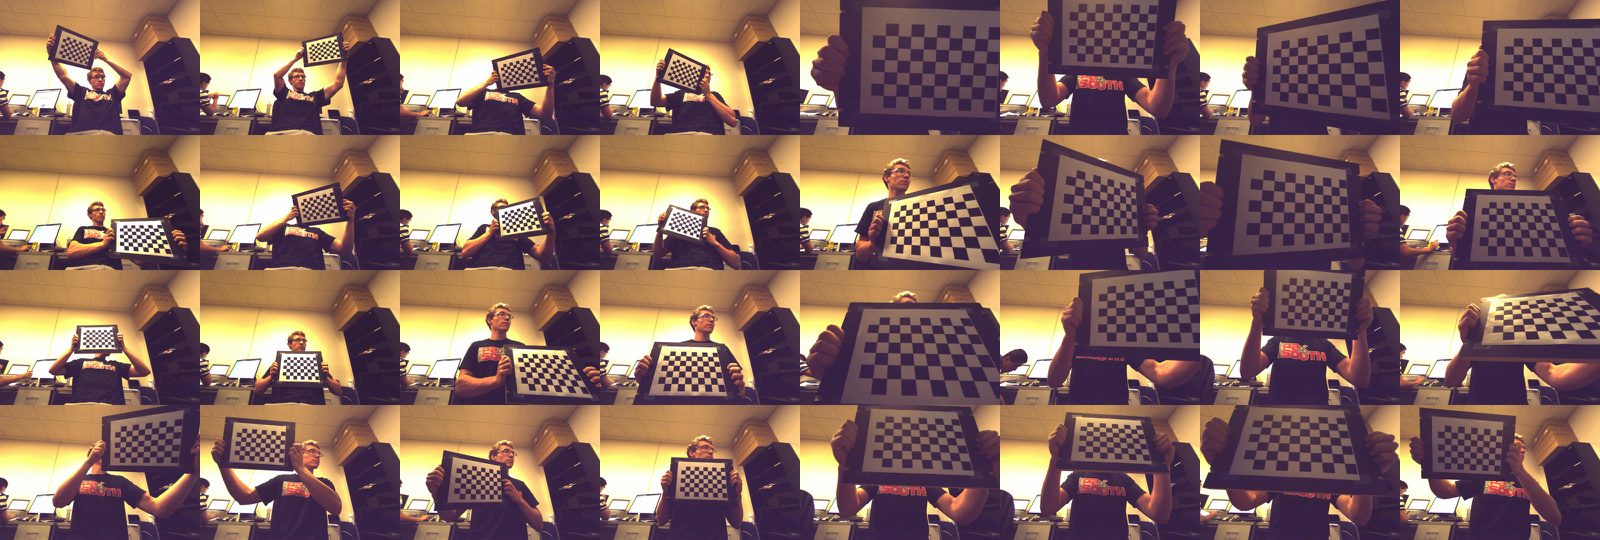
\includegraphics[width=.9\textwidth]{figures/combine_images_final.jpg}}
		%\end{tabular}
	\end{center}
	\caption{A collection of good viewing angles and distances for a calibration board}
	\label{fig:goodAngles}
\end{figure*}

When collecting images using a calibration target there are a number of important factors to consider. The input images should show the calibration board at a variety of locations, depths, and angles. Fig. \ref{fig:goodAngles} shows a collection of images taken when calibrating the stereo rig shown in Fig. \ref{fig:sensors}. The calibration was performed using the OpenCV fisheye camera calibration functions. This set of images highlights the important lessons learned. First there are views of the board from different distances, from far to near as seen left to right respectively. Second, 
the board is skewed with respect to the image plane; this is achieved by tilting the target to be non parallel to the camera. Third, the board should never be rotated past 90 degrees otherwise the images can be flipped; it is worth noting that using an odd by even dimension calibration pattern makes the board robust to orientation changes. The pattern should be visible in the field of view in its entirety, although this is an obvious point, when there are no preview capabilities it can be challenging. In particular, when calibrating a stereo system the pattern should be fully visible in both the left and the right camera.

\begin{figure*}[ht]
	\begin{center}
		\leavevmode
		\begin{tabular}{ccc}
			\subfloat[]{\fbox{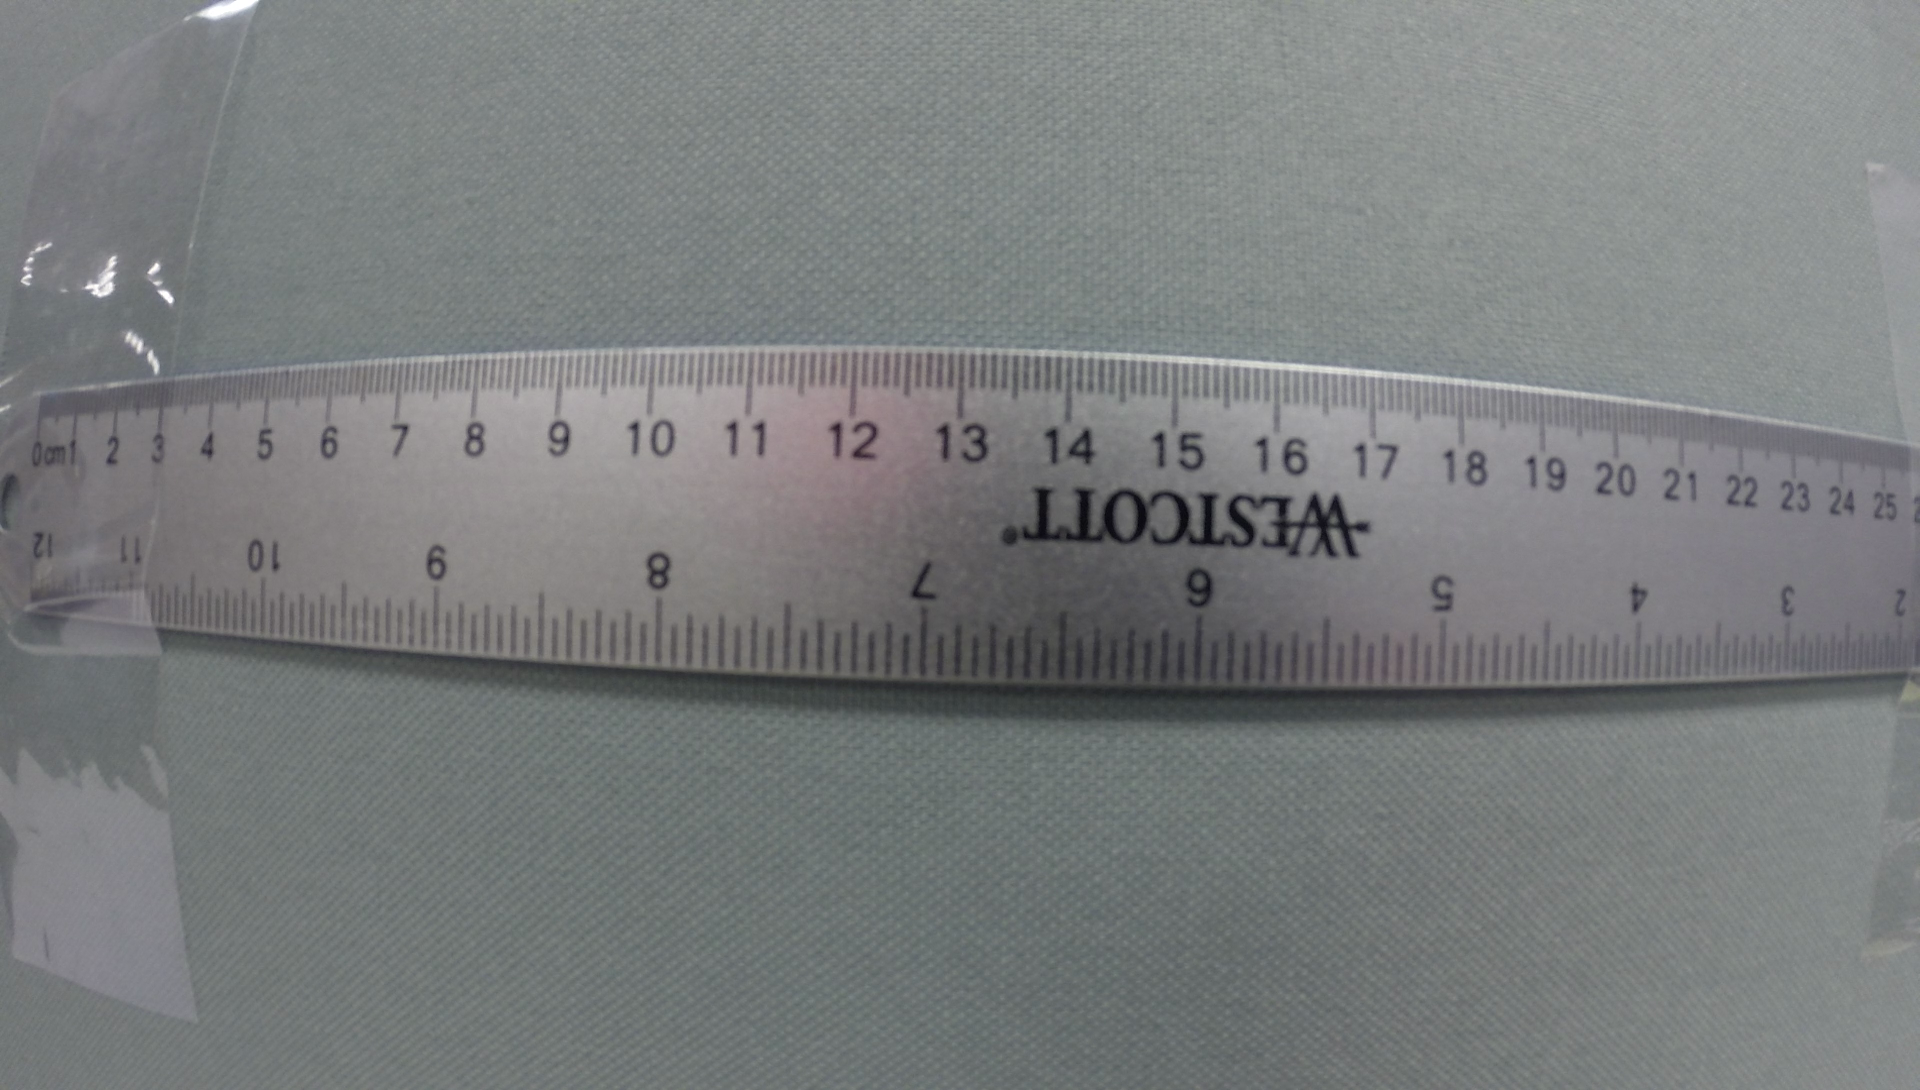
\includegraphics[width=.4\textwidth]{figures/without_superview.png}\label{fig:withouts}}} &
			\subfloat[]{\fbox{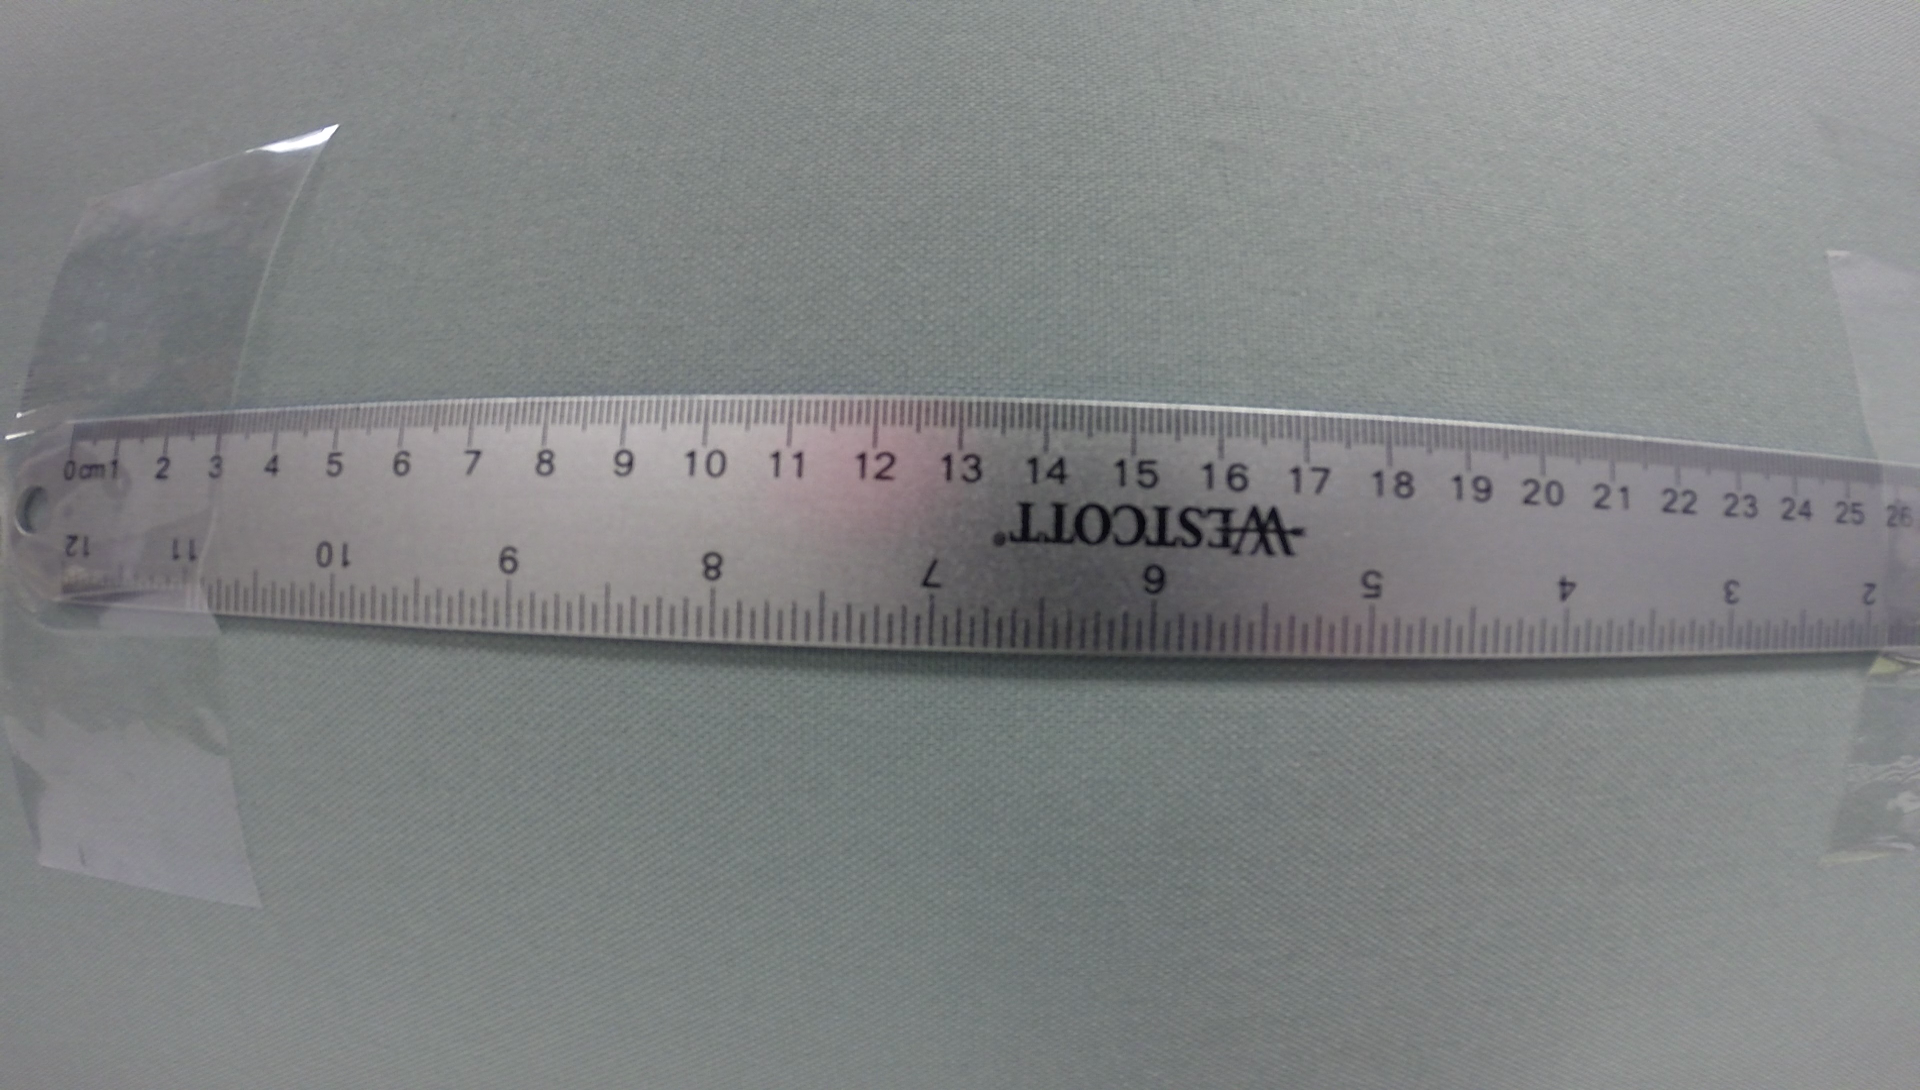
\includegraphics[width=.4\textwidth]{figures/with_superview.png}\label{fig:withs}}}&
		\end{tabular}
	\end{center}
	\caption{From the same camera pose, (a) 1080p GoPro footage without the SuperView feature. (b) 1080p GoPro footage with the SuperView feature.}
	\label{fig:comparisons}
\end{figure*}